We perform three sets of experiments to evaluate the model and the stochastic variational inference proposed. 
First, we use a toy problem to demonstrate the effectiveness of the proposed method in learning the model parameters.
Second, we assess the predictive accuracy of the model on two medium-sized datasets and compare with existing multiple output models.
In the final experiments, we evaluate the model on large-scale learning with multiple tasks.

\subsection{TOY PROBLEM}
In this toy problem we use two related outputs generated from the same latent function $sin(x)$ but are corrupted by independent noises: $y_1(x) = sin(x) + \epsilon$ and $y_2(x) = -sin(x) + \epsilon$, $\epsilon \sim \Normal(0,0.01)$.
Each output has missing values in one region of the input space.
% Say that this is from a single gpsvi
The predictive distributions of the model compared to that of independent GPs with stochastic variational inference are shown in figure \ref{fig:toy}.
Furthermore, the inference algorithm correctly learns the correlation between the two functions giving weights $w_{11} = 1.07$ and $w_{21} = -1.06$.

\begin{figure*}
\centering
\begin{tabular}{cccc}
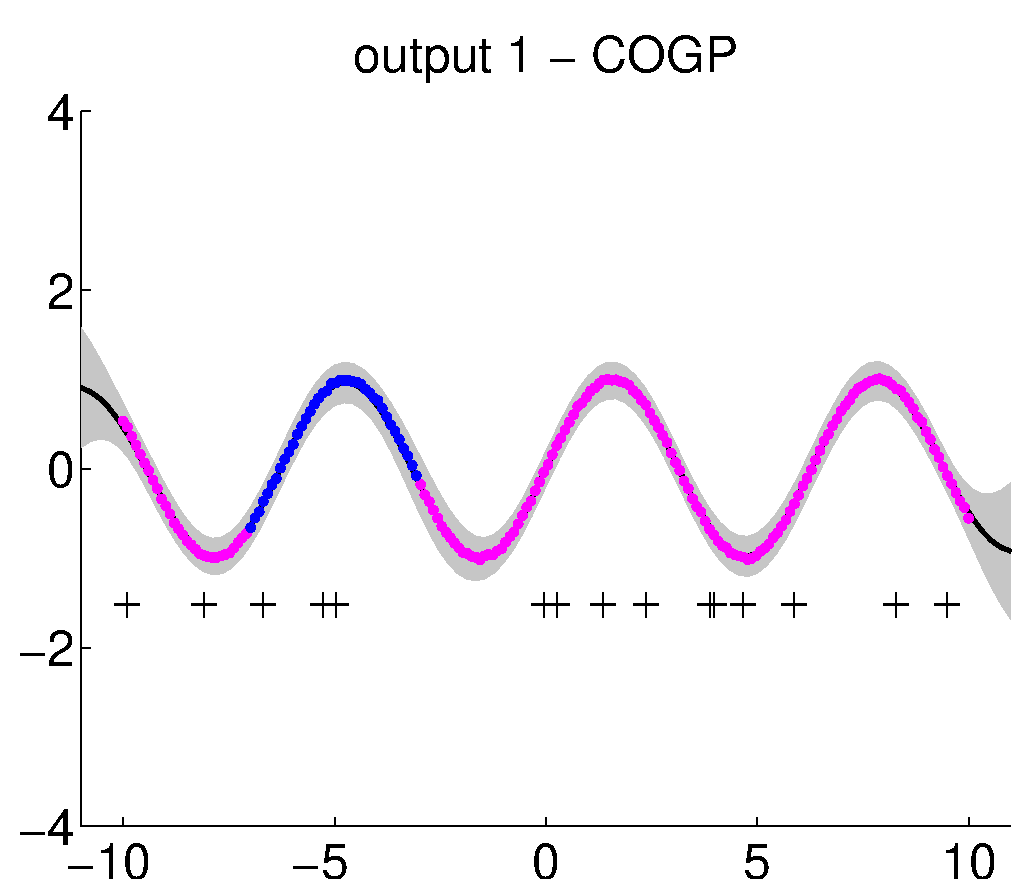
\includegraphics[scale=0.25]{figures/toy-slfm-y1.eps} &
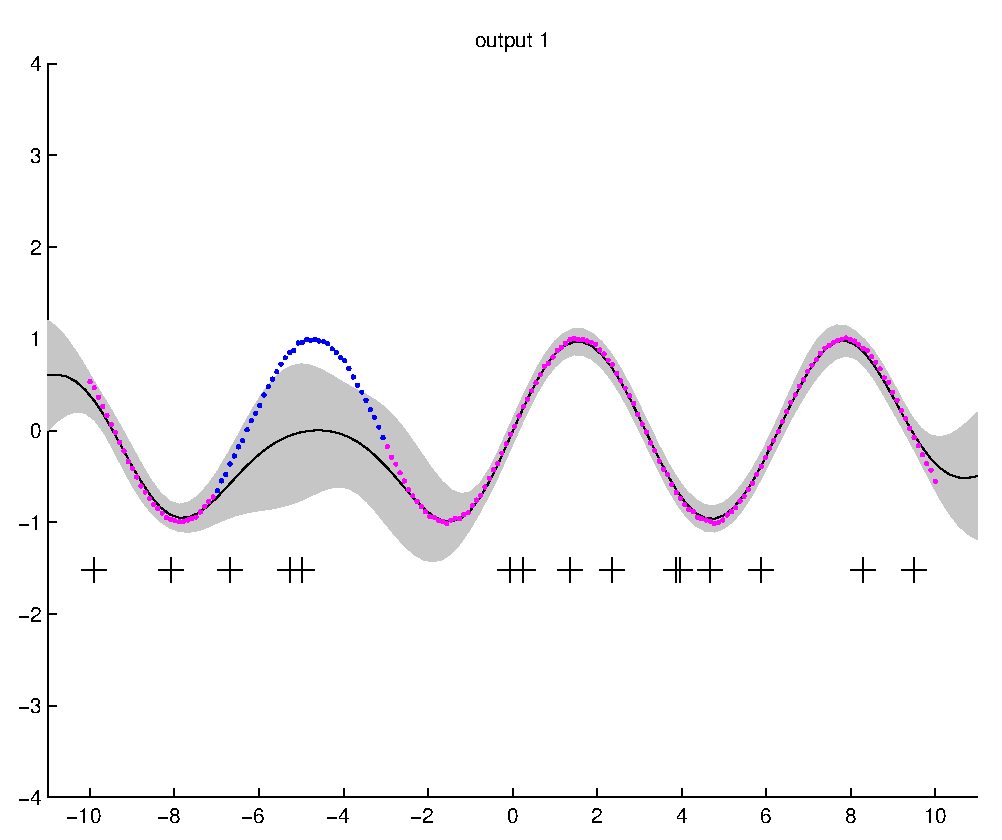
\includegraphics[scale=0.25]{figures/toy-svigp-y1.eps} &
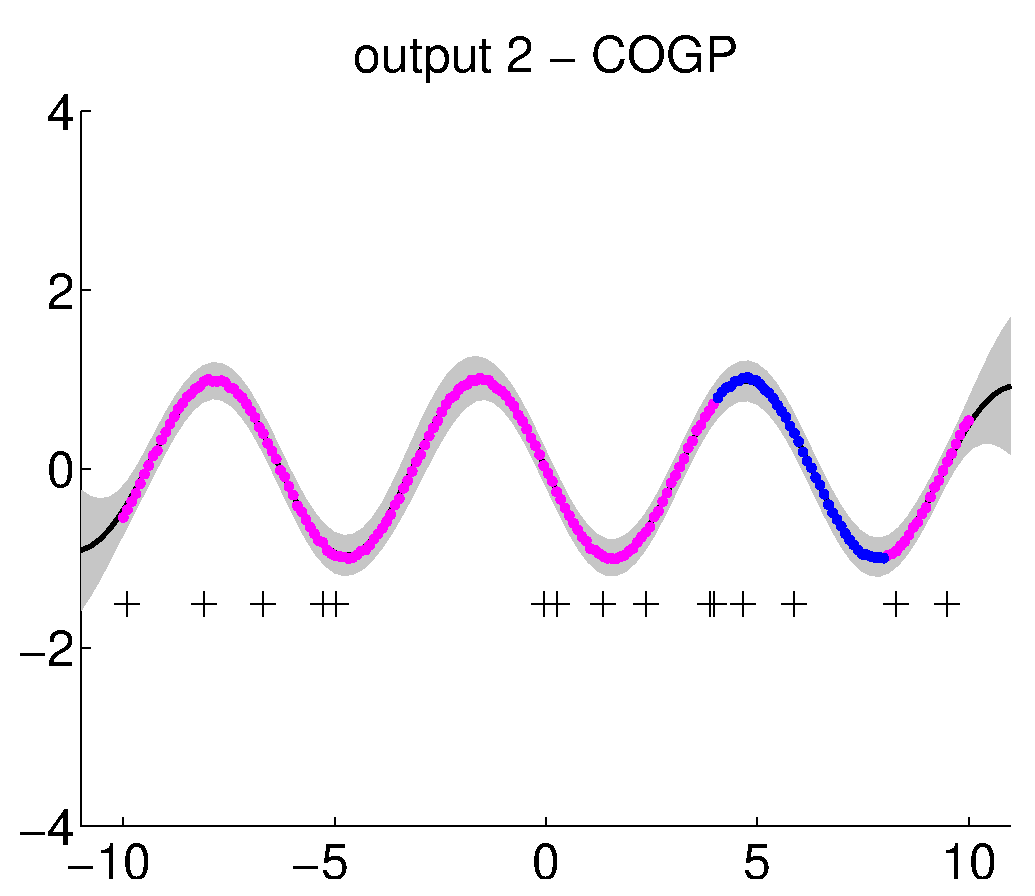
\includegraphics[scale=0.25]{figures/toy-slfm-y2.eps} &
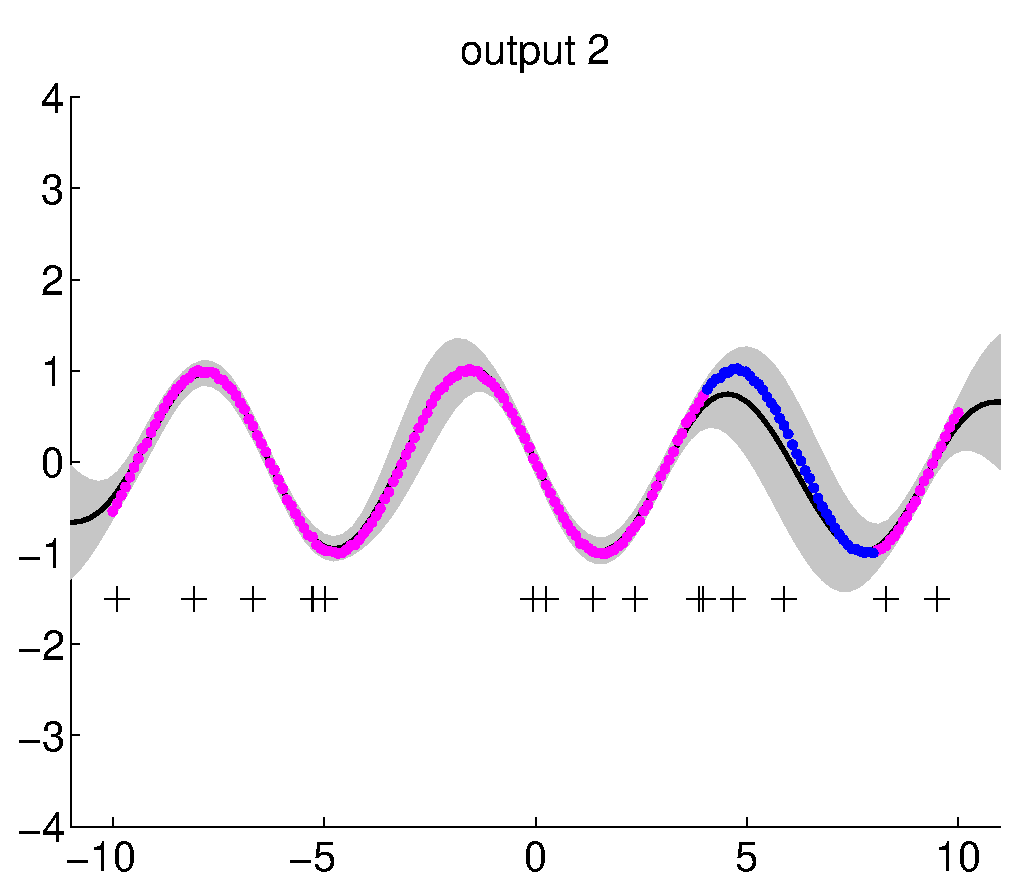
\includegraphics[scale=0.25]{figures/toy-svigp-y2.eps}
\end{tabular}
\caption{Predictive distributions of the multioutput GPs (first and third figure) and independent GPs using stochastic variational inference (second and last figure) for the  toy problem. Solid black line: predictive mean; grey bar: two standard deviations; magenta dots: real observations; blue dots: missing data. The black crosses show the locations of the inducing inputs.}
\label{fig:toy}
\end{figure*}

\subsection{EVALUATION OF THE PREDICTIVE ACCURACY}
\subsubsection{Foregin Exchange Rate Prediction}
In this experiment we predict the foreign exchange rate.
The smse are shown in Table \ref{tab:fx}.

\begin{table}[h]
\caption{Performance comparison by SMSE on the fx dataset.}
\label{tab:fx}
\begin{center}
\begin{tabular}{c|c}
method & smse \\ \hline
SLFM (Q=2) & 0.2232 \\
SLFM (Q=1) & 0.48 \\
CGP & 0.2795 \\
ICM & 0.3927
\end{tabular}
\end{center}
\end{table}

\begin{figure*}
\centering
\begin{tabular}{ccc}
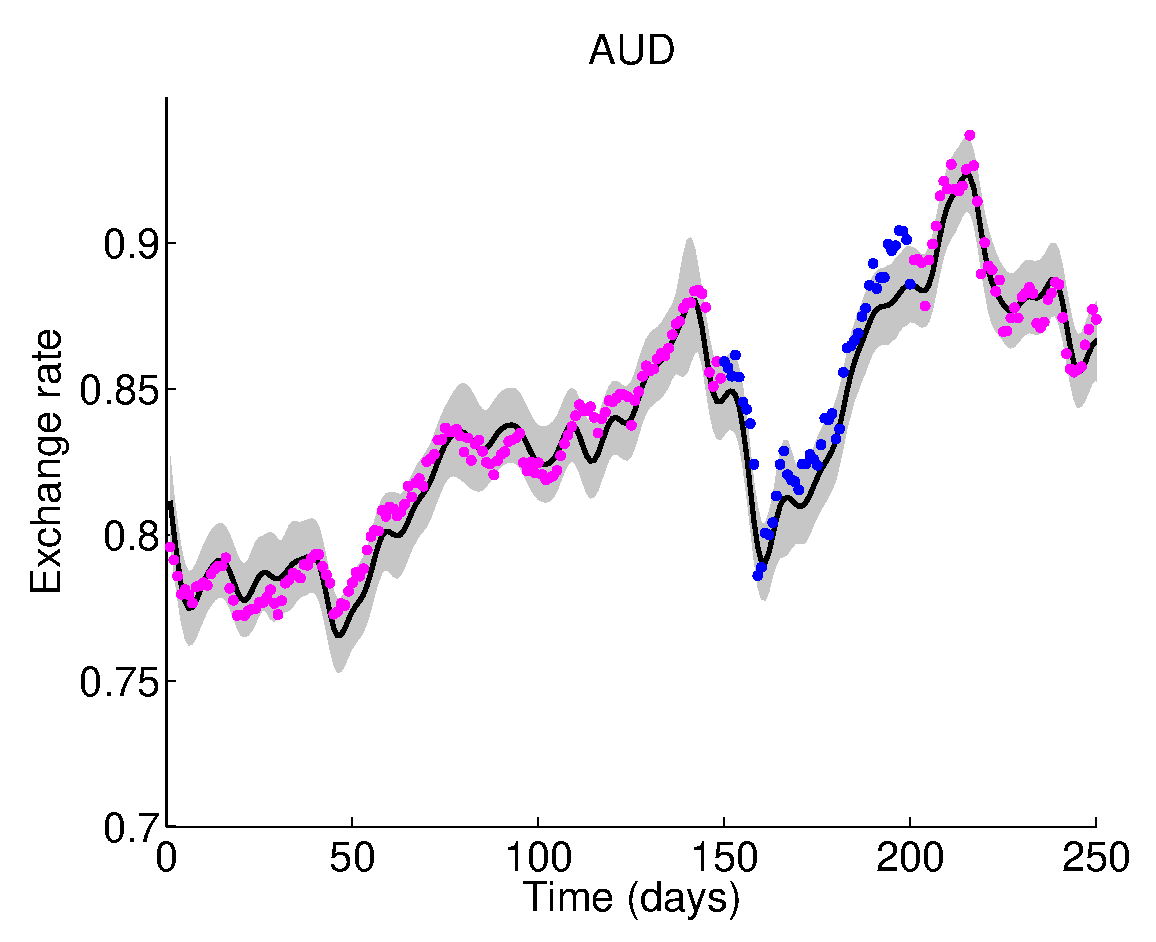
\includegraphics[scale=0.3]{figures/fxAUD.eps} &
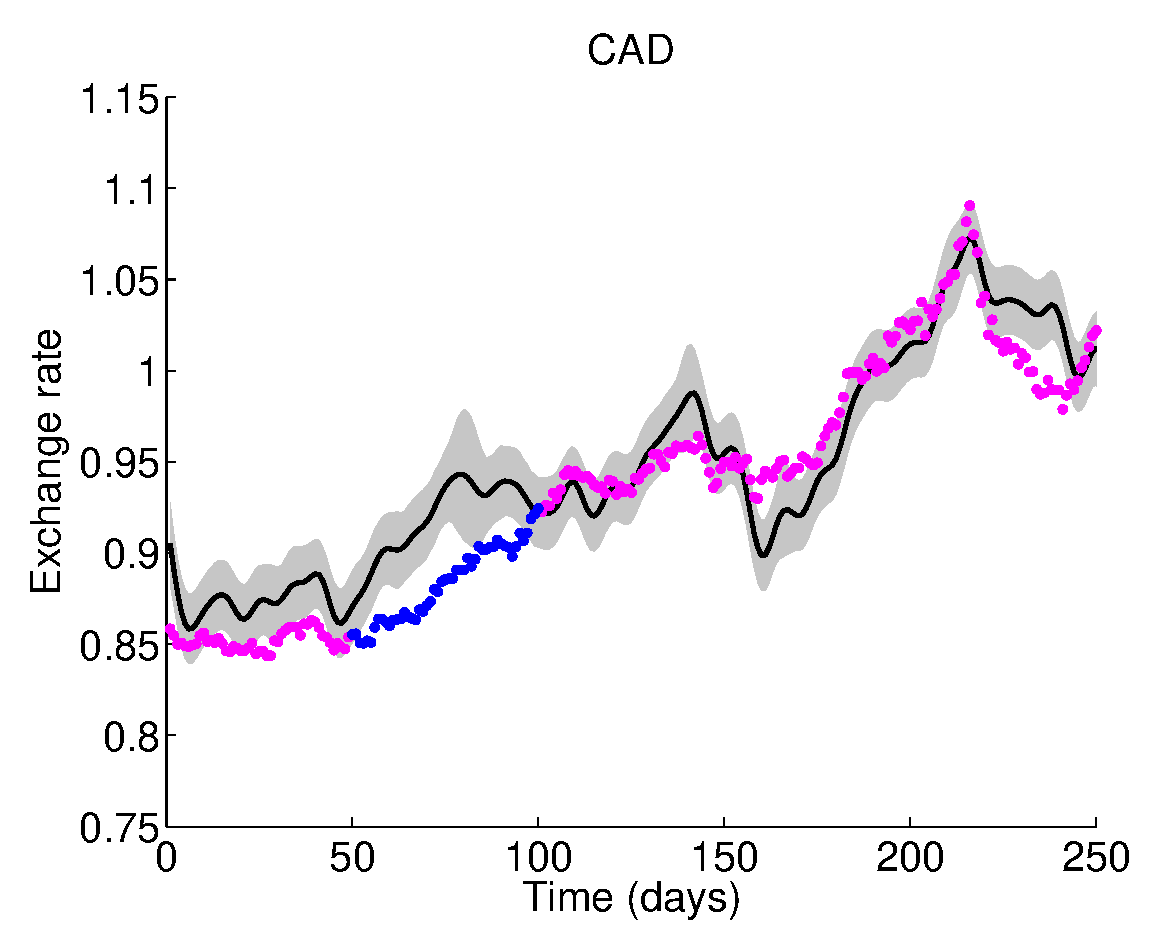
\includegraphics[scale=0.3]{figures/fxCAD.eps} &
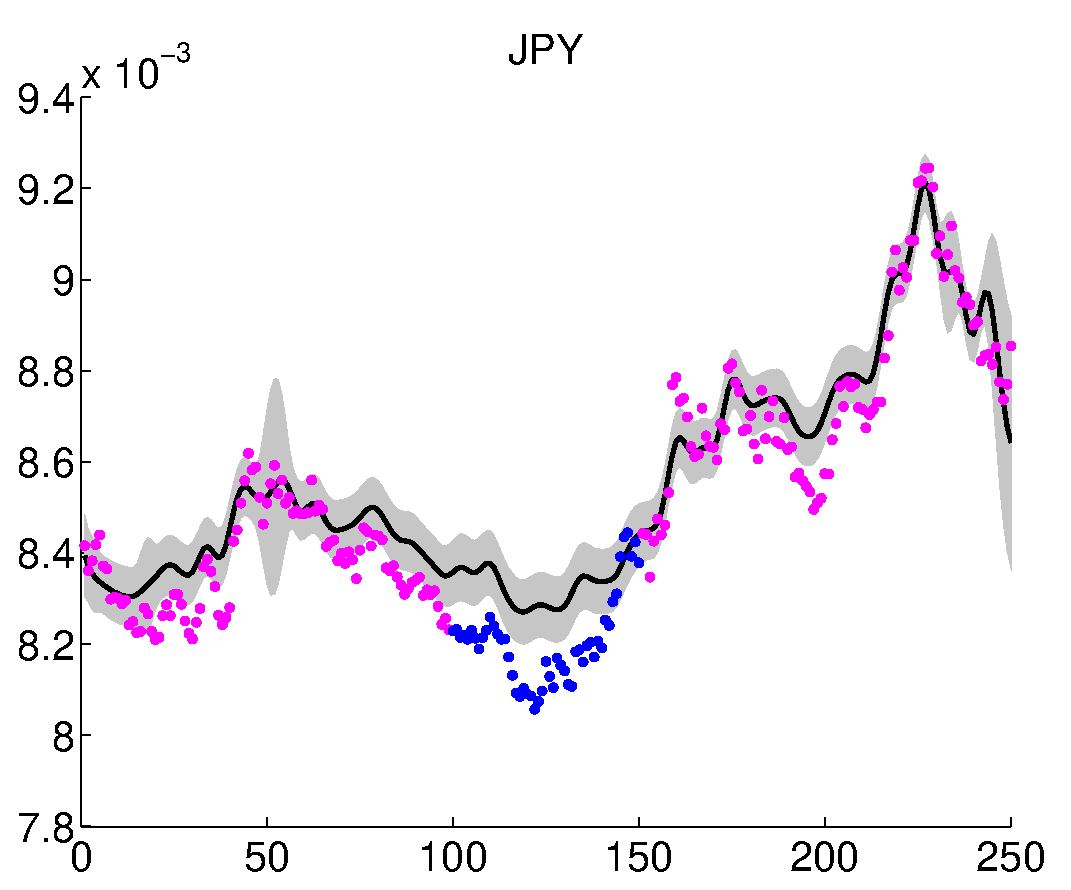
\includegraphics[scale=0.3]{figures/fxJPY.eps}
\end{tabular}
\caption{Real observations and predictive distributions for AUD (left), CAD (middle), and JPY (right). The color coding scheme is the same as in figure \ref{fig:toy}.}
\label{fig:fx}
\end{figure*}

\subsubsection{Weather Data Prediction}

\begin{figure*}
\centering
\begin{tabular}{cc}
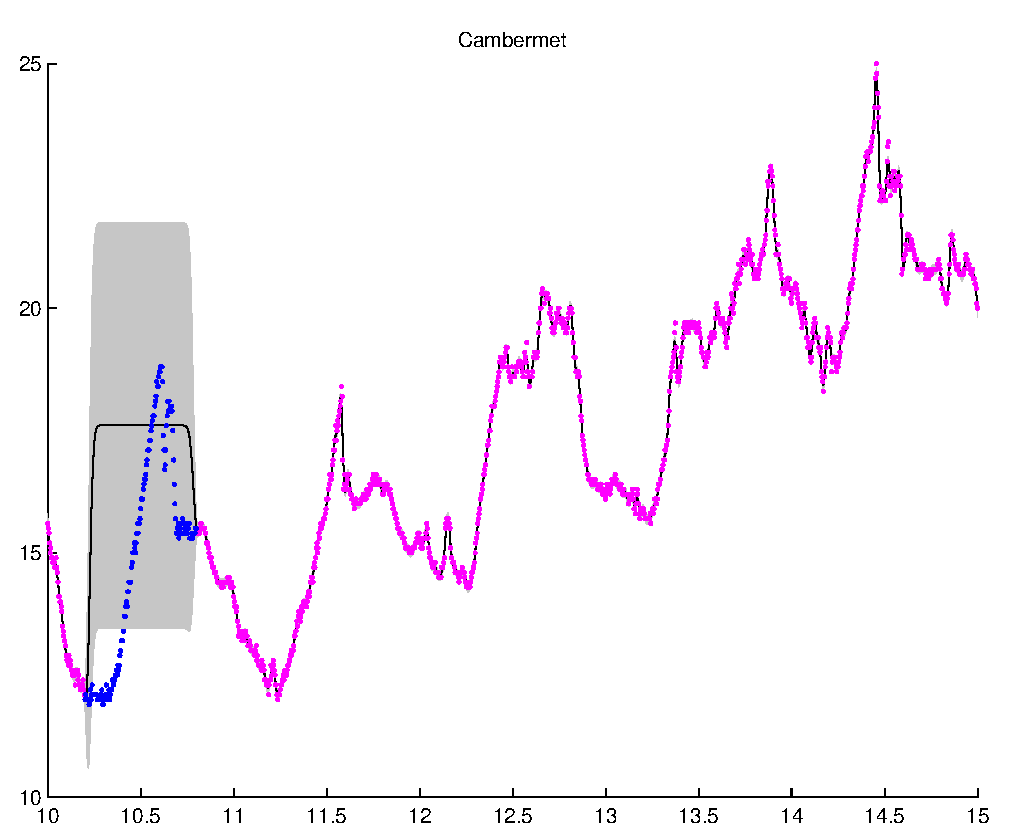
\includegraphics[scale=0.3]{figures/weatherCambermet.eps} &
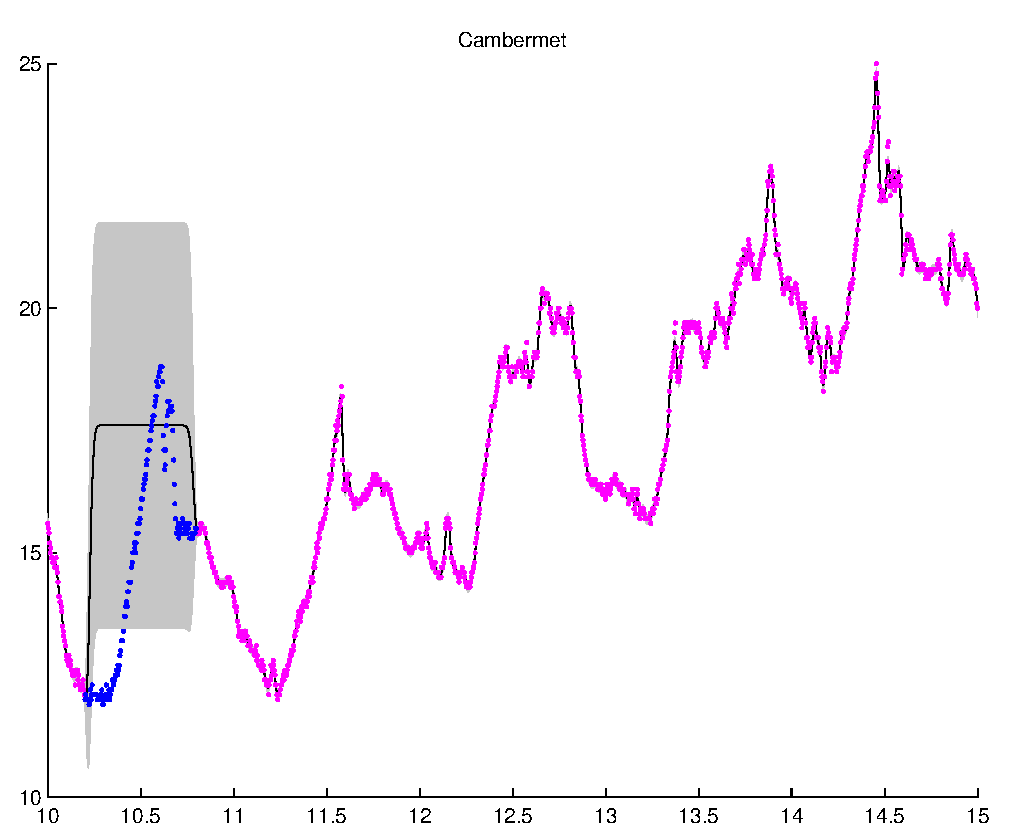
\includegraphics[scale=0.3]{figures/weatherCambermet.eps} \\
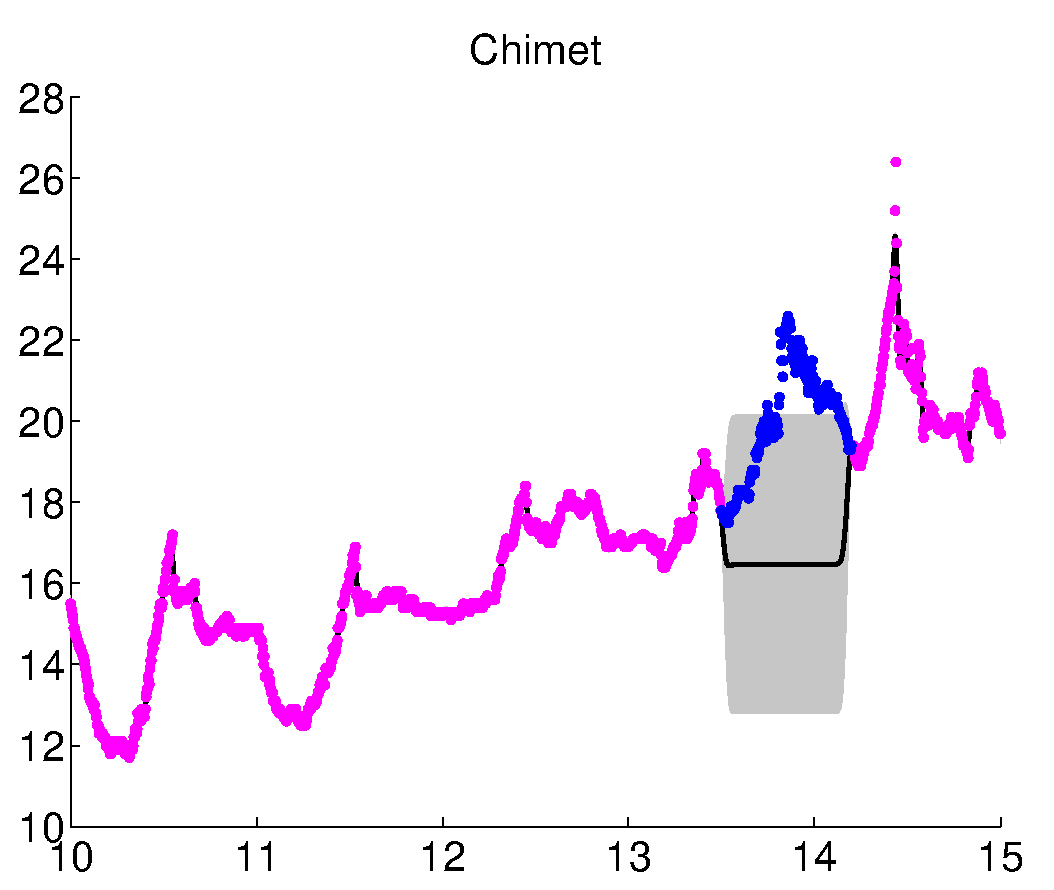
\includegraphics[scale=0.3]{figures/weatherChimet.eps} &
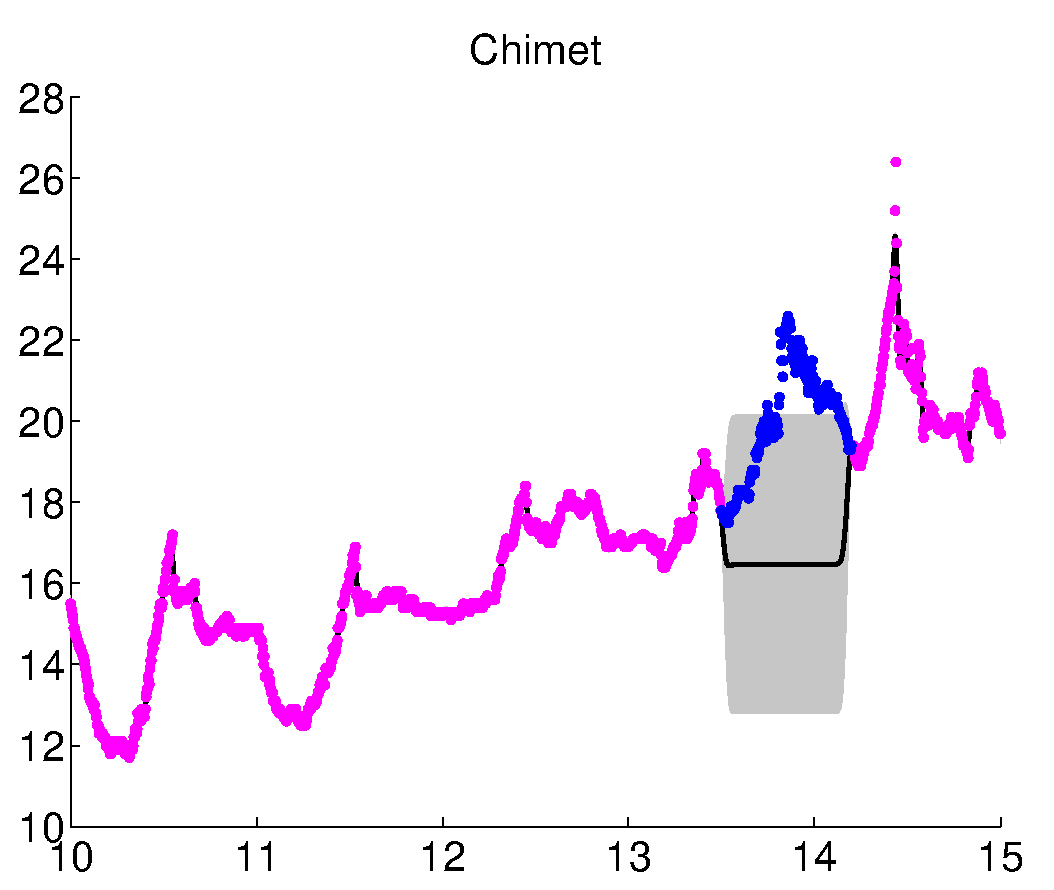
\includegraphics[scale=0.3]{figures/weatherChimet.eps}
\end{tabular}
\caption{Predictive distributions of the multioutput GPs (left column) and full independent GPs (right column) for the air temperature problem.}
\label{fig:toy}
\end{figure*}

\subsection{LARGE-SCALE EXPERIMENTS}
\subsubsection{Robort Arms}
\subsubsection{Foreign Exchange Rate Prediction}
